
%\documentclass[landscape]{slides}
\documentclass{beamer}
\usepackage{beamerfoils}
\usetheme{Pittsburgh}
%\usepackage[accumulated]{beamerseminar}
                                % remove ``accumulated'' option
                                % for original behaviour
%\usepackage{beamerthemeclassic}
\usepackage{ulem}
%\usepackage{beamerthemesplit}

%\usepackage{beamerthemeshadow}

%\usepackage{beamerthemeplain}
%\usepackage{times}
\usepackage{colortbl}

%\usepackage{lslide}
\def\emptyline{\vspace{10pt}}
\usepackage{amssymb}
%\usepackage{french}
%\usepackage[latin1]{inputenc}
\usepackage[utf8]{inputenc}
%\usepackage[T1]{fontenc}
\usepackage[]{color}
%\usepackage[usenames,dvipsnames]{color}
%\usepackage[pdftex]{color}
%\usepackage[]{colorlslide,epsfig}
%\usepackage{amsfonts,stmaryrd}
\usepackage{epsfig}

\usepackage{graphicx,array}
\usepackage{tikz}
\usetikzlibrary{shadows.blur}
\usepackage{amsmath}%,amsthm}
\usepackage{hyperref}
\usepackage{pifont}

%\renewcommand{\frame}{\end{slide}   \begin{slide}}
%\newcommand{\frametitle}{\centerline}
 

%\usepackage{beamerthemeshadow}
\usepackage{graphicx}
%\usepackage{beamerthemesplit}

\graphicspath{{./}{figures/}}

%%%%%%%%%%%%%%%%%% ENVIRONMENTS %%%%%%%%%%%%%%%%%%%%%%%%%%%%%%%%%%%%%%%%%%%%%%%%%
\newtheorem{deft}{Definition}
%\newtheorem{theorem}{Théorème}
\newtheorem{proposition}{Proposition}
\newtheorem{exemple}{Example}
\newtheorem{postulat}{Postulate}


%%%%%%%%%%%%%%%%%% COLORS %%%%%%%%%%%%%%%%%%%%%%%%%%%%%%%%%%%%%%%%%%%%%%%%%%%%%%%
%\definecolor{coltitle}{rgb}{0.1, 0.1, 0.543}
%\definecolor{colitemi}{rgb}{0, 0.75, 0.99}
%\definecolor{colexemp}{rgb}{0.6, 0.4, 0}
%\definecolor{colmult}{rgb}{0, 1, 0}
%\definecolor{gris}{rgb}{0.8, 0.8, 0.8}
\definecolor{encre}{rgb}{0.2, 0, 0.4}
\definecolor{lightblue}{rgb}{0.3,0.35,5}
% Colors for Adleman's classification diagram
\definecolor{adlemanblue}{RGB}{30,30,120}
\definecolor{adlemangray}{RGB}{192,192,192}
%\definecolor{grisbleu}{rgb}{0.8, 0.8, 1}
%\definecolor{cadre}{rgb}{0.7, 0.7, 0.7}
%\definecolor{cadresubsec}{rgb}{0, 0.3, 0.3}
%\definecolor{cadreombre}{rgb}{0.8, 0.8, 0.8}
%\definecolor{colsection}{rgb}{0.4, 0.2, 0.2}

%\definecolor{bleur}{rgb}{0.3, 0, 0.6}
%\definecolor{bleuv}{rgb}{0, 0.3, 0.6}
%\definecolor{rougeb}{rgb}{0.6, 0, 0.3}
%\definecolor{rougev}{rgb}{0.6, 0.3, 0}
%\definecolor{rougealert}{rgb}{1., 0.2, 0}
%\definecolor{vertr}{rgb}{0.3, 0.6, 0}
%\definecolor{vertb}{rgb}{0, 0.6, 0.3}
%\definecolor{blanc}{rgb}{1, 1, 1}

\newcommand{\red}[1]{\only<#1>{\color{red}}}
\newcommand{\green}[1]{\only<#1>{\color{green}}}
\newcommand{\lra}{\leftrightarrow}
\newcommand{\Fd}{\mathbb{F}}
\newcommand{\enlight}[1]{\textit{\color{blue}#1}}
\newcommand{\blue}[1]{\textit{\color{blue}#1}}

%%   for the headline etc.
\renewcommand\normalcolor{\color{coltitle}}


%%   for the background
%\pagecolor{grisbleu}
%%   for the text
\color{encre}

%%%%%%%%%%%%%%% style settings ....
 \beamertemplatenavigationsymbolsempty
\beamertemplatefootempty
%\beamertemplatefootframenumber
\setbeamertemplate{footline}[frame number]


\title{Malware - Overview}

\AtBeginSection[]
{
\begin{frame}
\frametitle{Outline}
\tableofcontents[currentsection,sectionstyle=show/shaded,subsectionstyle=show/show/hide]
\end{frame}
}

\AtBeginSubsection[]
{
\begin{frame}
\frametitle{Outline}
\tableofcontents[currentsubsection,sectionstyle=show/shaded,subsectionstyle=show/shaded/hide]
\end{frame}
}
%%%%%%%%%%%%%%%%%%%%%%%%%%%%%%%%%%%%%%%%%%%%%%%%%%%%%%%%%%%%%%%%%%%%%%%%%%%%%%%%%%
\titlegraphic{
\centering

\includegraphics[width=4cm]{logo-upvd.png}\\[0.3cm]

\includegraphics[width=6cm]{../../Cours/Chap01-Logiciels-Malveillants/malware1.jpg}
}
\begin{document}

\maketitle


\section{Introduction - Taxonomy}

\subsection{Definition and Classification}



\begin{frame}
\frametitle{Definition of Malware}

%\begin{deft}[Malware]
 \begin{block}{Definition (Malware):}
  A \enlight{simple program} or \enlight{self-replicating program}:
\begin{itemize}
\item  with offensive intent, installing itself in an information system without the user's knowledge,
\item designed to compromise the confidentiality, integrity, or availability of that system,
  \item or capable of falsely incriminating its owner or user in criminal activity.
\end{itemize}
\end{block}
%\end{deft}

\end{frame}



\begin{frame}

\begin{postulat}
Malware can affect any environment capable of code execution!
\end{postulat}

\begin{itemize}
\item All operating systems.
\item Mobile environments (smartphones, gaming consoles, GPS devices, embedded computers\ldots).
\item Many document formats.
\end{itemize}
\end{frame}

\begin{frame}
\frametitle{Adleman's Classification}

Adleman classified malicious software into 4 categories.

\begin{center}
\begin{tikzpicture}[
    bluebox/.style={rectangle, rounded corners=10pt, fill=adlemanblue, text=white,
                    minimum height=1cm, minimum width=2.4cm, align=center, font=\footnotesize\bfseries,
                    blur shadow={shadow blur steps=5, shadow xshift=0.5mm, shadow yshift=-0.5mm}},
    graybox/.style={rectangle, rounded corners=10pt, fill=adlemangray, text=black,
                    minimum height=1cm, minimum width=3cm, align=center, font=\footnotesize\bfseries,
                    blur shadow={shadow blur steps=5, shadow xshift=0.5mm, shadow yshift=-0.5mm}},
    connector/.style={line width=1.8pt, rounded corners=8pt, draw=black!70}
]
    % Level 1 - Root
    \node[bluebox, minimum width=3cm] (malware) at (0,0) {Malware};

    % Level 2
    \node[graybox] (simple) at (-3,-2) {Simple Programs};
    \node[graybox, minimum width=3.2cm] (selfrep) at (3,-2) {Self-Replicating\\Programs};

    % Level 3
    \node[bluebox] (logic) at (-4.3,-4) {Logic Bombs};
    \node[bluebox] (trojan) at (-1.6,-4) {Trojan Horses};
    \node[bluebox] (virus) at (1.6,-4) {Viruses};
    \node[bluebox] (worm) at (4.3,-4) {Worms};

    % Connections with rounded corners
    \draw[connector] (malware.south) -- ++(0,-0.5) -| (simple.north);
    \draw[connector] (malware.south) -- ++(0,-0.5) -| (selfrep.north);
    \draw[connector] (simple.south) -- ++(0,-0.5) -| (logic.north);
    \draw[connector] (simple.south) -- ++(0,-0.5) -| (trojan.north);
    \draw[connector] (selfrep.south) -- ++(0,-0.5) -| (virus.north);
    \draw[connector] (selfrep.south) -- ++(0,-0.5) -| (worm.north);
\end{tikzpicture}
\end{center}

The main distinction is:
\begin{itemize}
\item \enlight{Simple program}: a standard program with malicious intent.
\item \enlight{Self-replicating}: a program that copies its own code, typically into other executables.
\end{itemize}
\end{frame}

\subsection{Logic Bomb}

\begin{frame}
\frametitle{Logic Bomb}

\begin{deft}[Logic Bomb]
A logic bomb is a simple malicious program that installs itself in a system and waits for a specific event (date, action, particular data...) called a \blue{trigger} to execute its offensive function.
\end{deft}


These programs often constitute the payload of a virus (e.g., the CIH virus that activates every April 26th).
\end{frame}


\begin{frame}
\frametitle{Logic Bomb Example}
\begin{itemize}
\item A system administrator had implanted a program that checked for the presence of his name in the company's payroll records.

\item If his name was absent (indicating termination), the program would encrypt all company hard drives.
  \begin{center}
    
\includegraphics[width=5cm]{../../Cours/Chap01-Logiciels-Malveillants/encrypted-hard-drive.jpeg}
    \end{center}
\item Without the encryption key, the company could no longer access its data.
\end{itemize}
\end{frame}

\begin{frame}
\frametitle{Limitations of Antivirus Protection Against Logic Bombs}
\begin{itemize}
\item Antivirus software struggles to detect logic bombs, as they appear to be ordinary programs.
\item Advanced antivirus techniques (heuristic analysis, code emulation) are inherently limited against unknown logic bombs.
\end{itemize}
\end{frame}


\subsection{Trojan Horses}

\begin{frame}
\frametitle{Trojan Horses}

\begin{deft}[Trojan Horse]
A Trojan horse is a simple program composed of two parts:
\begin{itemize}
\item the server module:
  \begin{itemize}
  \item Installed on the victim's computer.
    \item  Covertly provides the attacker with access to all or part of the system resources over the network.
    \end{itemize}
\item  the client module:
  \begin{itemize}
  \item  Located on the attacker's machine.
    \item Allows access to services unknowingly provided by the victim.
    \end{itemize}
\end{itemize}




\end{deft}

\end{frame}



\begin{frame}
\frametitle{Trojan Horses}
{\color{blue} The server module:}
\begin{itemize}
\item Usually hidden within another \textit{\color{blue} harmless and attractive program.}
  \item Executing this program installs the Trojan's server component without the victim's knowledge.
\end{itemize}
\pause
{\color{blue} The client module:}
\begin{itemize}
\item Scans the network for IP addresses and ports (TCP or UDP) of machines infected by the server module.
  \item Takes control of the infected machines found.
%\item This control allows the attacker to carry out offensive actions.
\end{itemize}
\end{frame}


\begin{frame}
\frametitle{Client-Server Architecture in Trojan Horses}


\includegraphics[width=10cm]{../../Cours/Chap01-Logiciels-Malveillants/client-serveur}

\end{frame}

\begin{frame}
\frametitle{Trojan Horse Detection}

Detection of these programs is inconsistent.
\begin{itemize}
\item A well-crafted Trojan horse not distributed on the internet has a high chance of evading antivirus detection.
  \bigskip
\item Using a firewall is highly recommended, although several techniques exist or are being developed to bypass them.
\end{itemize}
\end{frame}

\begin{frame}
\frametitle{Trojan Horse Examples}
\begin{itemize}
\item Decoys: programs mimicking the normal behavior of a legitimate system program (e.g., fake Unix login banner).
  \bigskip
\item Keyboard spies, known as \enlight{keyloggers}, are a specific type of Trojan horse.
\end{itemize}
\bigskip
The offensive action typically involves stealing one or more pieces of information from the victim's machine.
\end{frame}





\subsection{Viruses and Worms}
\begin{frame}
\frametitle{Worms and Viruses: Definitions}
\begin{deft}[Virus] A program that propagates by copying its own code.
\end{deft}

\begin{deft}[Worm] Can be viewed as a network-oriented virus. The main difference from a virus is that a worm is not necessarily attached to a file (e.g., simple worms like Slammer).
\end{deft}
\end{frame}

\begin{frame}
\frametitle{Computer Worms}

Three main classes of worms:
\begin{itemize}
\item {\color{lightblue} Simple worms.} Exploit security vulnerabilities (Slammer, Sasser,\ldots).
\item {\color{lightblue} Macro worms.} Use social engineering and infected office document attachments.
\item {\color{lightblue} Email worms.} Use social engineering and infected executable attachments (Bagle, Netsky,\ldots).
\end{itemize}

\end{frame}


\begin{frame}
In the following sections, we will focus primarily on self-replicating programs:
\begin{itemize}
\item We will mainly study viruses,
\item and to a lesser extent, worms.
\end{itemize}
\end{frame}

\section{Virus Fundamentals}

\subsection{Propagation and Life Cycle}

\begin{frame}
\frametitle{Propagation Method}
%\begin{enumerate}
% \item
  The malicious program is carried by a host program or \enlight{dropper}.
  % (called infected program; in the case of the first infection carried out by the attacker, the term \enlight{dropper} is used).
  \bigskip

  {\color{blue} When the \enlight{dropper} is executed:}
\begin{enumerate}
\item The malicious program (or viral code) takes control:
  \begin{itemize}
  \item It operates according to its own mode.
  \item The host program is temporarily suspended.
  \end{itemize}
  \medskip

\item It returns control to the host program, which then executes normally without revealing the presence of the malicious code.
\end{enumerate}
%\end{enumerate}

\end{frame}


\begin{frame}
\frametitle{Functional Diagram of a Virus}

\begin{enumerate}
\item A \enlight{search} routine to find target programs.
%\begin{itemize}
%\item Verification that the file is executable and has the correct format.
%\item Verification that the file is not already infected (\enlight{reinfection control}).
%\end{itemize}
%This part determines its effectiveness in terms of reach and speed.
\medskip
\item A \enlight{copy} routine: injection of viral code into the target.
  \medskip
\item An \enlight{anti-detection} routine. Purpose: to counter antivirus action.
  \medskip
\item The \enlight{payload}, possibly coupled with a delayed activation mechanism (\enlight{trigger}).% This is what causes harm.
\end{enumerate}
\end{frame}


\begin{frame}
\frametitle{Life Cycle of a Virus or Worm}

Three phases can be identified in the life of a virus:
\begin{itemize}
\item The infection phase.
\item The dormant phase (incubation).
\item The execution phase (payload activation).
\end{itemize}

%\enlight{Distribution}: once the virus is incorporated into an \textit{innocuous} program, the dropper, the programmer will use programs adapted to the virus depending on the target(s):
%\begin{itemize}
%\item For a limited number of victims: prior intelligence is required.
%\item Infected games or humor-based software.
%\end{itemize}
\end{frame}


\begin{frame}
\frametitle{Infection Phase}

During this phase, the virus spreads through the environment:
\begin{itemize}
\item \enlight{Passively}
\begin{itemize}
\item  The infected medium is copied to a storage device (CD-ROM, download site, forum,\ldots) and transmitted.
  \medskip
\item Victims can then copy and execute it in their own environment.
\end{itemize}
\medskip

\item \enlight{Actively}
\begin{itemize}
\item  The user executes the dropper or a file already contaminated during a previous infection.
  \end{itemize}
\end{itemize}
% This phase differentiates simple infections from viruses: the duplication of code.
\end{frame}

\begin{frame}
\frametitle{Infection Phase}
During this phase, the virus searches for target programs: %which will in turn be infected
\begin{itemize}
\item An effective virus will verify that the file is executable, has the correct format, and that the target is not already infected.
\item It also ensures to minimize detection risks: for example, infection of *.COM executables must not exceed 64KB (maximum size of *.COM files).
\end{itemize}

The virus then copies its own code into the target.

\end{frame}



\begin{frame}
\frametitle{Dormant Phase (Incubation)}
\begin{itemize}
\item This is the longest part of a virus's life.
\item Primary mission: ensure the virus's survival.
\item The goal is to limit or prevent its detection:
\begin{itemize}
\item Detection by the user: by avoiding, for example, execution errors.% that could alert the user.
  \bigskip
\item Detection by antivirus: evading antivirus surveillance.

  %The virus will use several techniques to evade antivirus surveillance.
\end{itemize}
\end{itemize}
\end{frame}



\begin{frame}
\frametitle{Execution Phase (Payload Activation)}
During this phase, \enlight{the payload is activated}. Its triggering depends on its position: %. Its triggering mode depends on many factors and the location in the code where the routine is placed.
\begin{itemize}
\item \enlight{At the beginning of the code}: the payload will be executed before any infection. %This case is rare and generally limits the virus's or worm's survival phase.
\item \enlight{At the end of the code}: it will only occur after the infection process.
\item \enlight{In the middle of the code}: particularly if it is conditioned by the success or failure of the infection.
\end{itemize}
\end{frame}


\begin{frame}
  \frametitle{Execution Phase: Triggering}
  \begin{itemize}
\item Triggering can be delayed (trigger mechanism).

\item  The payload is then a logic bomb mounted on a viral vector.
  \end{itemize}
  \medskip

{\color{blue} Examples:}


\begin{itemize}
\item System date.
\item Number of infections completed.
\item A particular key sequence pressed a certain number of times (e.g., \texttt{CTRL+ALT+DEL}).
\item Number of times a \texttt{Word} document is opened.
\end{itemize}
%In fact, it all depends on the programmer's imagination and desired effects.
\end{frame}





\begin{frame}
\frametitle{Execution Phase: Payload Effects}
The effects of the payload are highly variable:
\begin{itemize}
\item \enlight{Non-destructive}: displaying images or animations, messages, ... % sound or music emission (playful or activist attack)
\item \enlight{Destructive}: the aim is to compromise
\begin{itemize}
\item  Data confidentiality (data exfiltration).
  \smallskip

\item  System or data integrity (file destruction/modification, ...) % random data modifications,\ldots)
  \smallskip

  \item System availability (CPU saturation, ...)
    \smallskip

  \item Data availability (encryption) or user incrimination.% (introduction of compromising data, ...))
\end{itemize}
\end{itemize}
\end{frame}


%\end{document}

\begin{frame}
\frametitle{Execution Phase: Hardware Destruction?}
\begin{itemize}
\item Generally not accepted by experts.
\item CIH controversy:
  \begin{itemize}
  \item CIH does not directly destroy hardware but the associated software (firmware, etc.).
  \item The hardware attack is only simulated.
  \end{itemize}
\item Other older examples: attacking floppy or hard disk drives through repeated I/O requests.
%\item These viruses target specific hardware and are therefore less detectable by antivirus software.
\end{itemize}
\end{frame}



\begin{frame}
\frametitle{Biological/Computer Comparison}
{\scriptsize
\begin{center}
\begin{tabular}{|c|c|}
\hline
Biological Virus & Computer Virus \\
\hline
\hline
Specific cell attacks & Specific format \\
by format & attacks \\
\hline
Infected cells & Infected program \\
produce new  & generates other \\
viruses & viral programs \\
\hline
Modification of cell's & Modification of \\
genetic information & program actions \\
\hline
Virus uses host cell & Multiplication only \\
structures to multiply & via infected program \\
\hline
Viral interactions & Binary viruses or anti-antivirus \\
Multiplication only & Execution required \\
in living cells & for dissemination \\
\hline
An infected cell & Reinfection prevention \\
is not reinfected & \\
by the same virus & \\
\hline
Retrovirus & Virus specifically targeting \\
& an antivirus - Source code virus \\
\hline
Viral mutation & Viral polymorphism \\
\hline
Healthy carrier & Latent viruses \\
\hline
Antigens & Signatures \\
\hline
\end{tabular}
\end{center}
}
\end{frame}





\subsection{Statistics and Metrics}


\begin{frame}
\frametitle{Some Statistics}
Statistics on malware are difficult to obtain and verify (...)

%\begin{itemize}
%\item The total number of known viruses was approximately 70,000 in January 2002.
%\item Each month, between 800 and 12,000 new viruses are discovered.
%\item In January, the distribution among different types of infections is given below.
%\end{itemize}


%$$diagram$$
\begin{center}
  %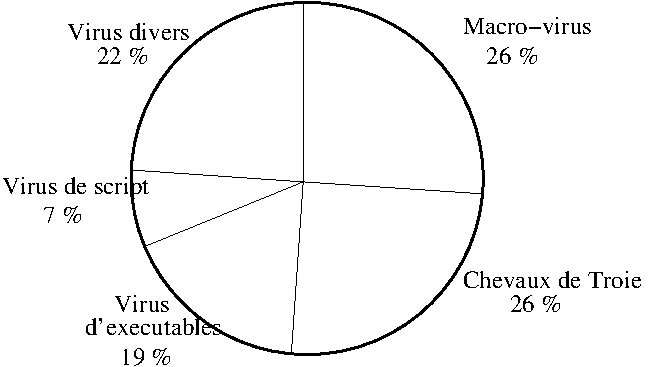
\includegraphics[width=4cm]{repartition-infection}
  
\includegraphics[width=6cm]{../../Cours/Chap01-Logiciels-Malveillants/progression-nb-malware.jpg} \vspace{0.2cm}
  
\includegraphics[width=4.5cm]{../../Cours/Chap01-Logiciels-Malveillants/repartition-malware-v1.png}
\end{center}


\end{frame}


%\begin{frame}
%\frametitle{Données et indices numériques, Virulence}

%\begin{deft}[Virulence]
%\begin{small}
%Soit $v$ un virus, on définit
%\begin{enumerate}
%\item L'indice infectieux $I^0_v$ d'un virus $v$ mesure le risque \enlight{a priori}.
%$$I^0_v = \frac{\mbox{Nombre de fichiers infectables par } v }{\mbox{Nombre total de fichiers du système}}$$
%\item L'indice infectieux $I^1_v$ d'un virus $v$ mesure le risque \enlight{a posteriori}.
%$$I^1_v = \frac{\mbox{Nombre de fichiers infectés par } v }{\mbox{Nombre  de fichiers infectables par } v}$$
%\item La virulence $V_v$ d'un virus $v$ est définit comme
%$$V_v = I^0_v \times I^1_v = \frac{\mbox{Nombre total de fichiers du système}}{\mbox{Nombre de fichiers infectés par } v }$$
%\end{enumerate}
%\end{small}
%\end{deft}
%\end{frame}


%\begin{frame}
%\frametitle{Données et indices numériques, Virulence}
%\begin{itemize}
%\item Fichiers considérés : uniquement fichiers exécutables ou fichiers documents (ps, pdf, word,\ldots).
%\item Ces indices ont un sens que dans un environnement bien défini (OS,etc.)
%\item Remarquons que les indices $I_v^0,I_v^1$ et $V_v$ ne considère que le risque d'infection et ne considère pas du t%out la charge finale.
%\item Ces indices sont relativement faciles à obtenir.
%\item Dans le cas des vers, les indices précédents sont définis en considérant non pas des fichiers mais des machines i%nfectées.
%\end{itemize}
%\end{frame}






%\begin{frame}
%\frametitle{Données et indices numériques - Détectabilité}

%\begin{small}
%\begin{proposition}[degré de détectabilité]
%Le degré de détectabilité d'une infection informatique  est inversement proportionnel à la durée de la phase d'incubation et proportionnel au nombre d'infections survenues dans ce système. Autrement dit
%$$\mbox{Détectabilité} = C \times \frac{\mbox{ Nombre de copies }}{\mbox{ Temps incubation }}$$
%où $0 \leq C \leq 1$. 
%\end{proposition}
%\begin{itemize}
%\item La constante $C$ décrit un certain nombre de paramètre : qualité de programmation, technique anti-antivirale, nat%ure de la charge finale.
%\item Cela permet donc de prendre en compte la totalité de l'activité du virus.
%\item Le degré de risque d'une infection informatique varie grosso modo inversement avec le degré de détectabilité de c%ette infection.
%\end{itemize}
%\end{small}
%\end{frame}



\section{Virus Infection Methods}

\subsection{Overwriting Viruses}


\begin{frame}
\frametitle{Overwriting Viruses}
When the virus executes:
\begin{itemize}
\item The search routine identifies targets.
\item Infection occurs by simply overwriting the target code with its own code.
\item These viruses generally lack a payload, as the infection method itself serves as one.
\end{itemize}
\end{frame}

\begin{frame}
\frametitle{Overwriting Viruses}

Three overwriting cases are possible:
\medskip

\enlight{\ding{202}} The virus overwrites the initial portion of the target code.

%\begin{itemize}
%\item L'en-tête spécifique de l'exécutable dont la fonction est de structurer les données est absent.
%\item Le code afin de faciliter la projection en mémoire par l'OS est alors absent.
%\item Le programme infecté ne pourra pas se lancer.
%\end{itemize}

\medskip


\enlight{\ding{203}} The virus overwrites the middle or terminal portion of the target code.
%\begin{itemize}
%\item Le virus doit alors installer une fonction de saut vers l'adresse de son %propre code en début du programme infecté s'il veut la main avant le programme cible.
%\item Selon les cas le programme cible ne se lancera pas et/ou son exécution avortera en cours de processus.
%\item  Dans ce cas on obtient une dose de furtivité : le dysfonctionnement est imputé par l'utilisateur à un boggue du programme plutôt qu'à un virus.
%\end{itemize}

%\end{frame}



%\begin{frame}
%\frametitle{Virus par écrasement de code}
\medskip

\enlight{\ding{204}} The virus simply replaces the target code with its own code. %Technique peu courante et facilement détectable puisque tous les exécutables infectés ont la même taille, et même code.

\begin{center}
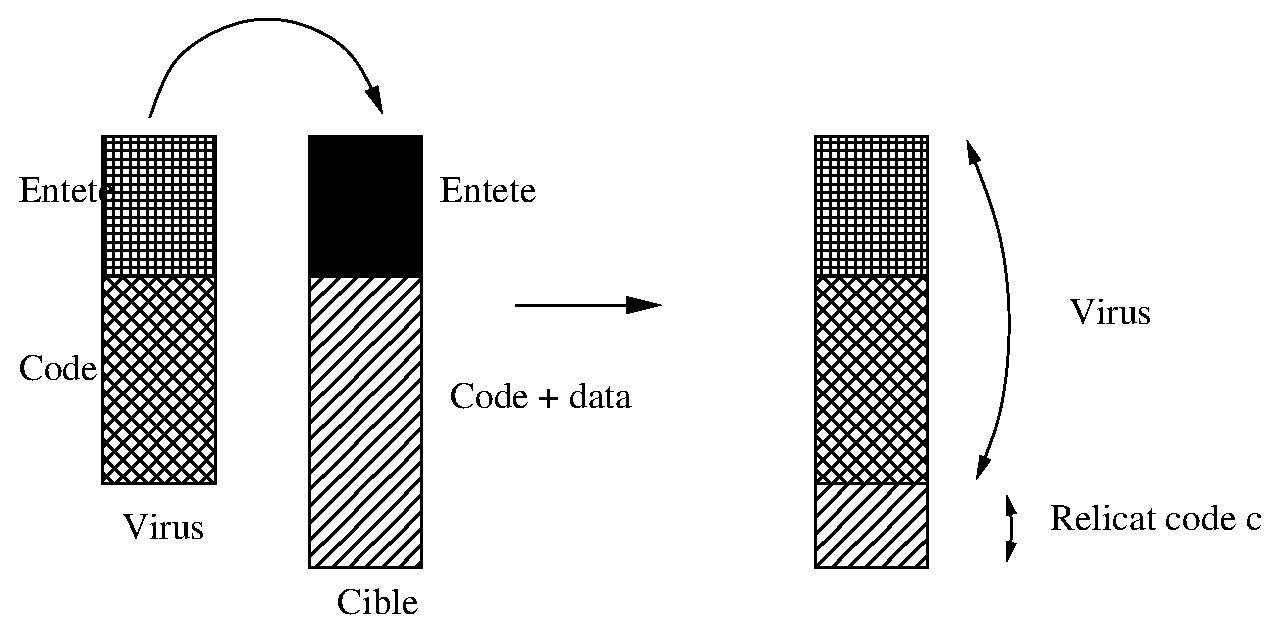
\includegraphics[width=8cm]{ecrasement}
\end{center}

\end{frame}





\subsection{Prepending and Appending Viruses (1/2)}

\begin{frame}

\frametitle{Prepending and Appending Viruses}

Viruses using this method attach their code to the target.
Two cases:
%Il en résulte une augmentation de la taille du programme infecté.


%Le virus a deux possibilités pour accoler son code :
\begin{itemize}
\item  \enlight{At the beginning of the target code (prepending).}% (type \textit{prepend} ou ajout en position initiale). C'est le cas le moins fréquemment réalisé car le plus compliqué.
This is complex because the header must be modified:% entre autre données
\begin{itemize}
\item File length and possibly code sections.
\item Address recalculation.
\item Additionally, a \enlight{jump} to the beginning of the target code must be added. % pour que le code cible s'exécute.
\end{itemize}

\end{itemize}
\end{frame}

\begin{frame}
\frametitle{Prepending and Appending Viruses (2/2)}
\begin{itemize}
\item \enlight{At the end of the target code (appending).}
\begin{itemize}
\item The beginning of the target code must be replaced with a jump to the viral code.
\item The replaced code must be executed at the end of the viral code.
\item Followed by a jump back to the target code.
\end{itemize}

\begin{center}
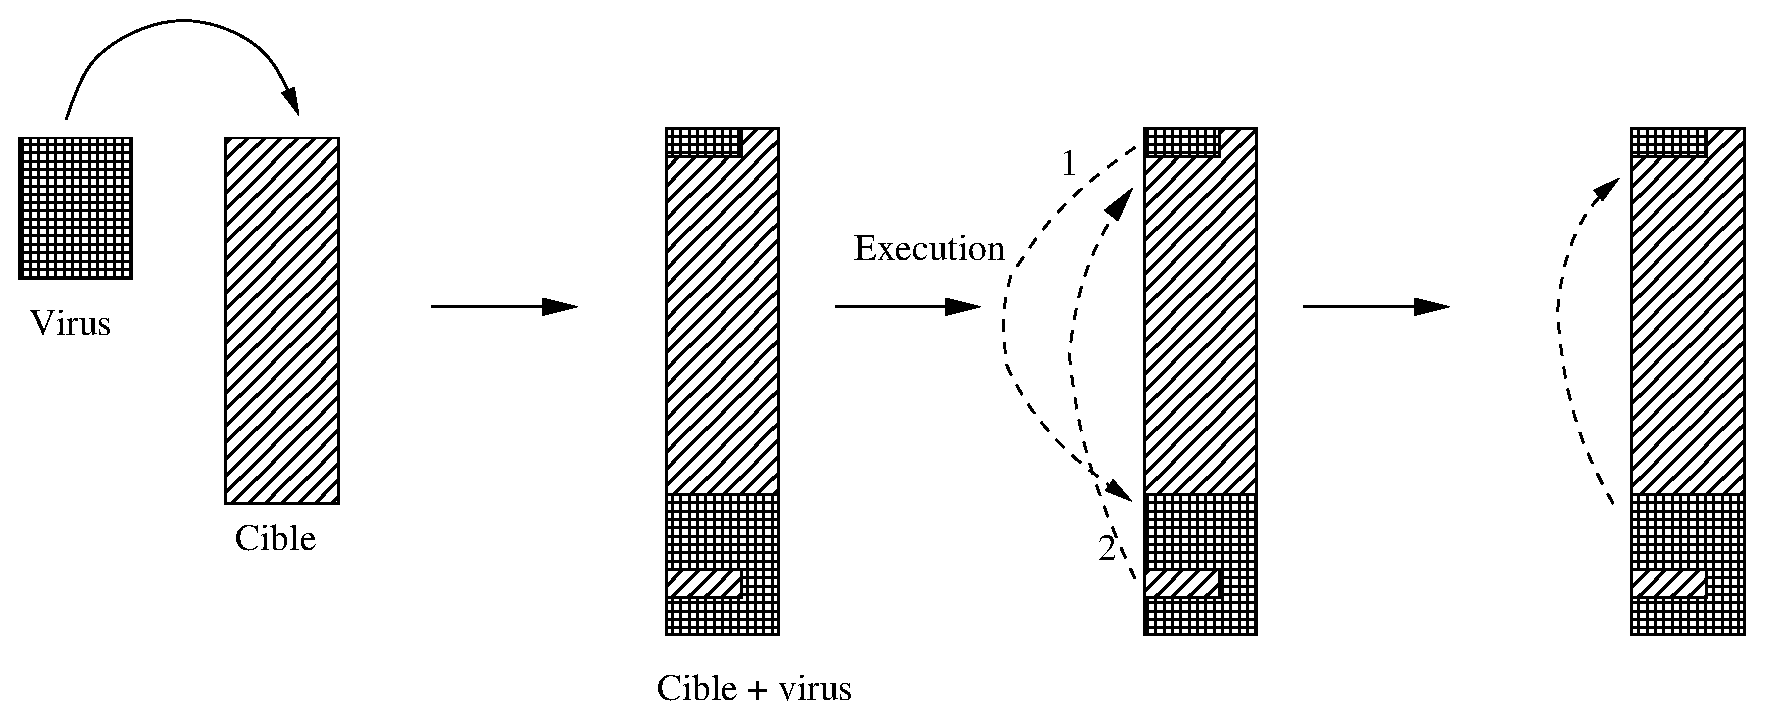
\includegraphics[width=10cm]{recouvrement}
\end{center}


\end{itemize}


\end{frame}

\subsection{Cavity Viruses}

\begin{frame}
\frametitle{Cavity Viruses}
These viruses primarily exploit the PE (Portable Executable) format of 32-bit Windows executables. This header enables during memory mapping:
\begin{itemize}
\item providing adequate information for memory installation (establishing a memory image);
\item allowing optimal sharing between multiple processes of EXE and DLL files.
\end{itemize}
This format lends itself particularly well to virus writing.
\end{frame}



%\begin{frame}
%\frametitle{Virus par  entrelacement  de code - fichier PE}
%Un fichier PE se compose
%\begin{itemize}
%\item D'une entête DOS qui permet de lancer le programme sous DOS et d'afficher le message indiquant que l'application ne fonctionne que sous Windows.
%\item De l'entête PE proprement dite. Il comprend deux structures de données essentielles, renseignées lors de la compilation et de l'édition dynamique et indispensables au lancement correct de l'application.
%\end{itemize}

%\end{frame}



%\begin{frame}
%\begin{columns}[c]
%\begin{column}{4cm} %{0.5\textwidth}
%\only<1>{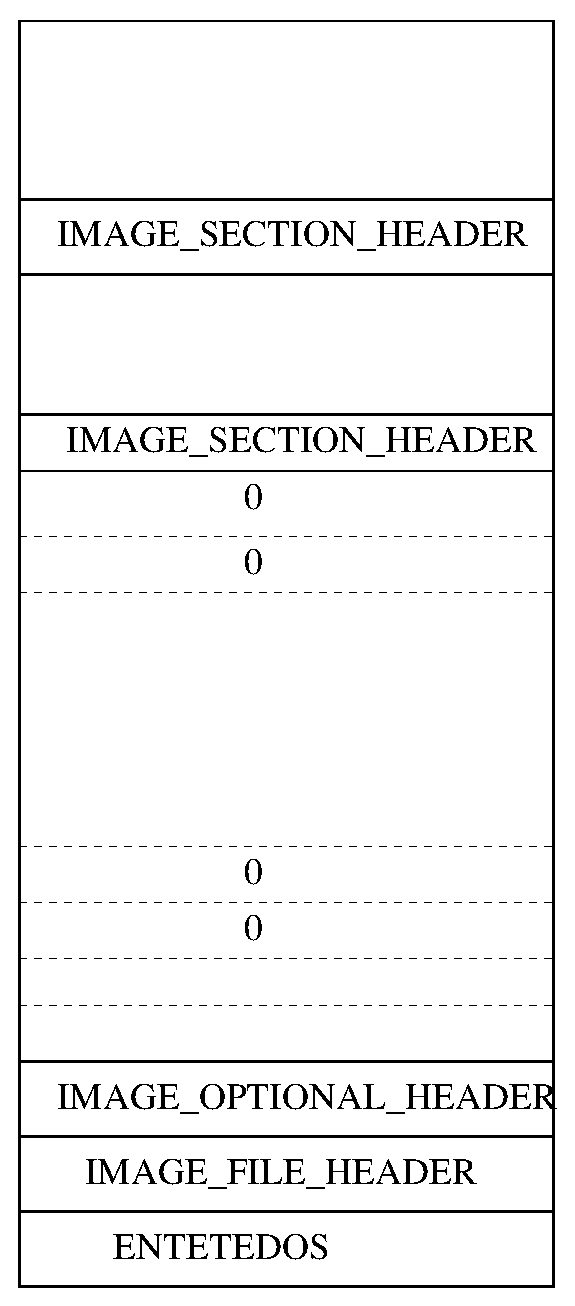
\includegraphics[width=4cm]{fichierPE}}
%\only<2>{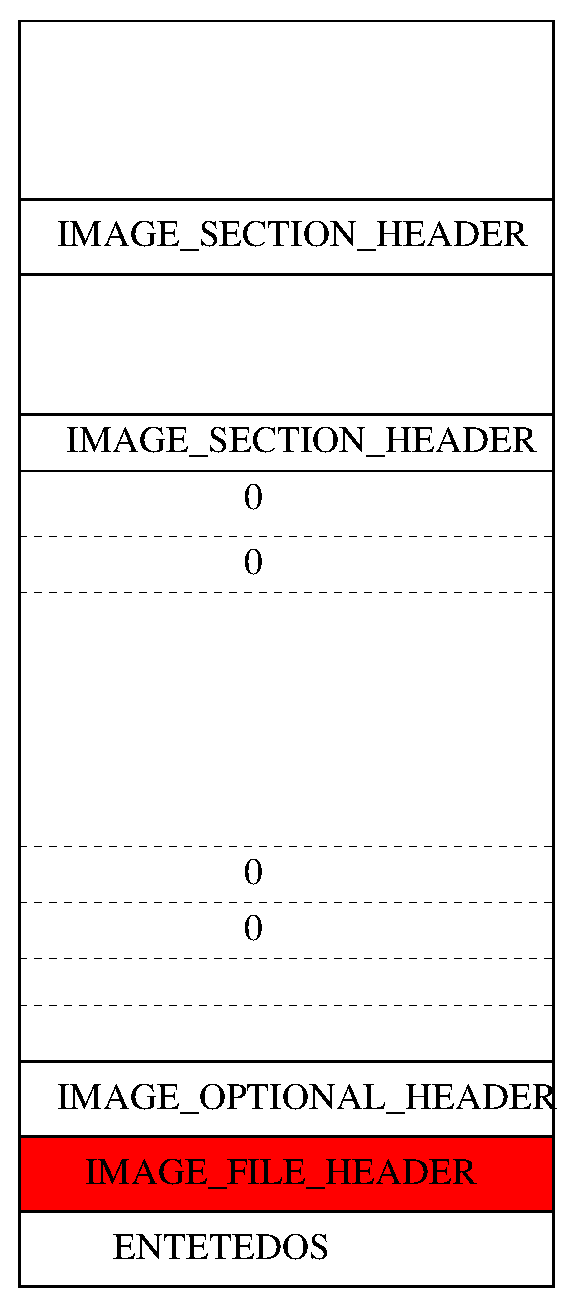
\includegraphics[width=4cm]{fichierPE-fileheader}}
%\only<3>{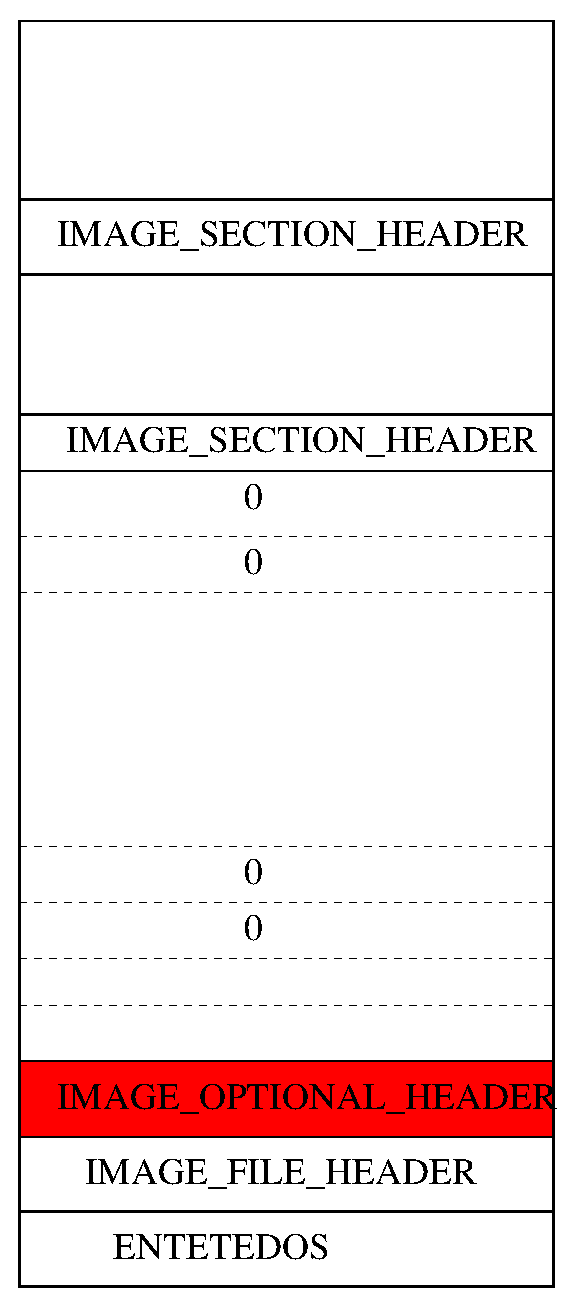
\includegraphics[width=4cm]{fichierPE-optionalheader}}
%\only<4>{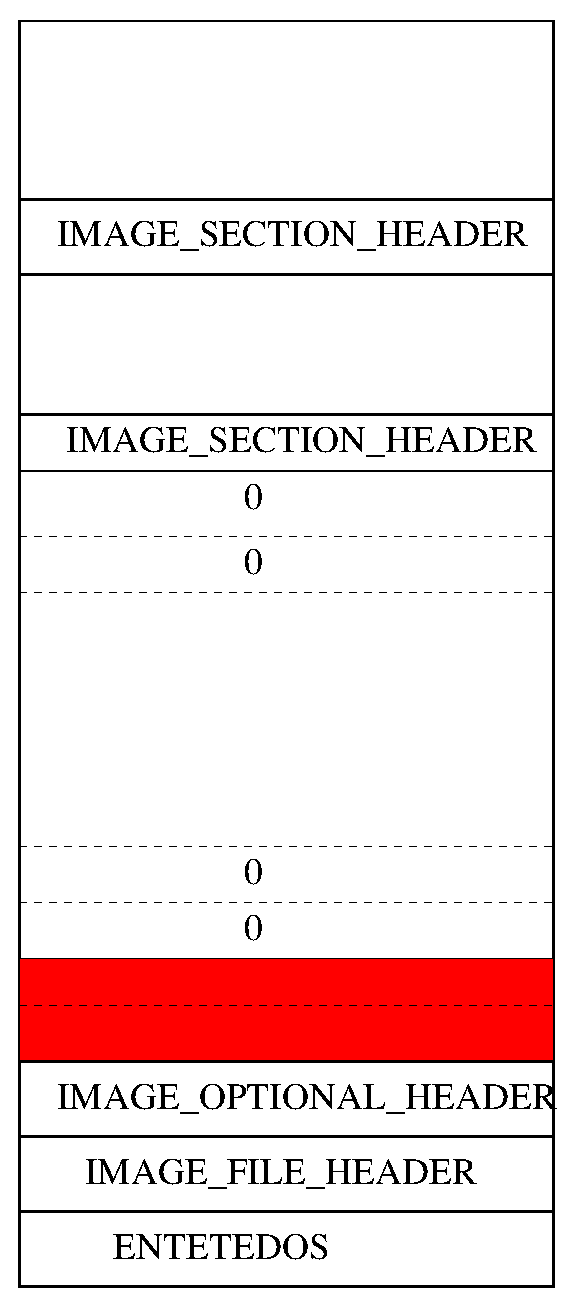
\includegraphics[width=4cm]{fichierPE-sectionheader}}
%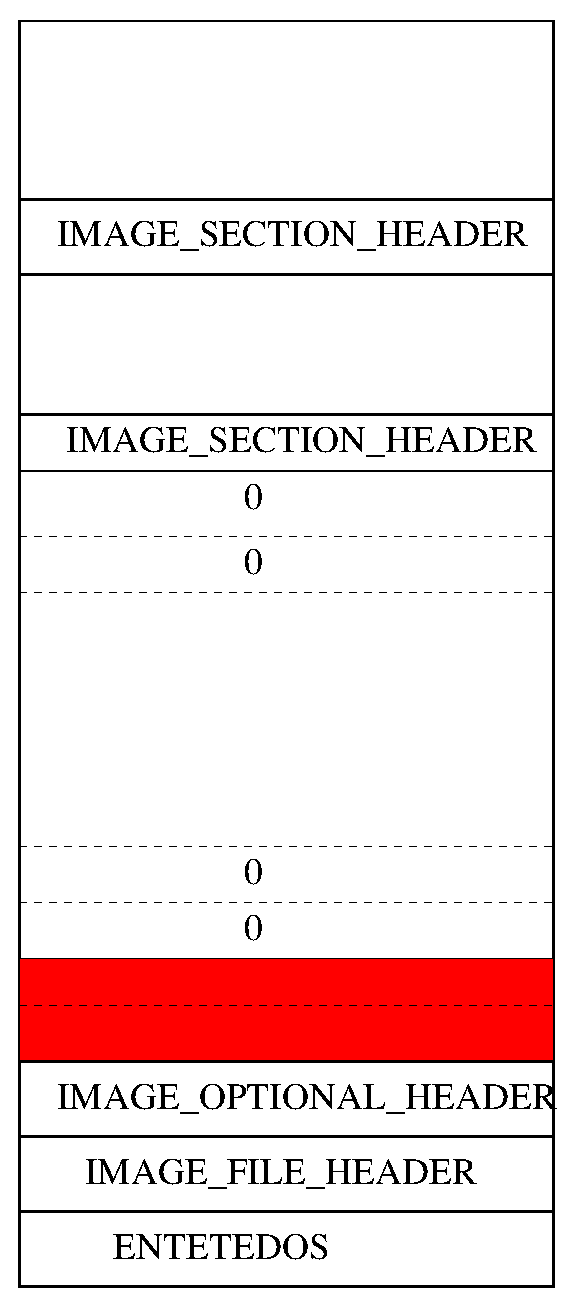
\includegraphics[width=4cm]{fichierPE-sectionheader}
%\end{column}

%\begin{column}[c]{6cm} 

%\only<2>{
% l'\texttt{IMAGE\_FILE\_HEADER} est 
%\smallskip


%\color{red}
%\begin{tt}
%\noindent typedef struct\{\\
%WORD Machine;\\
%WORD NumberOfSection;\\
%DWORD TimeDateStamp;\\
%DWORD PointerToSymbolTable;\\
%DWORD NumberOfSymbols;\\
%Word SizeOfOptionHeader;\\
%Word Characteristics;\\
%\} IMAGE\_FILE\_HEADER\\
%\end{tt}
%}

%\only<3>{\color{red}

%\begin{tt}

%\begin{small}
%\noindent typedef struct\{\\
%.... \\
%DWORD SizeOfCode;\\
%DWORD SizeOfInitializedData;\\
%DWORD SizeOfUnInitializedData;\\
%DWORD AddresOfEntryPoint;\\
%DWORD BaseOfCode;\\
%DOWRD BaseOfData;\\
%DWORD ImageBase \slash\slash adresse \\
%\qquad\qquad  \slash\slash de chargement\\
%DWORD SectionAlignment;\\
%....\\
%\} IMAGE\_OPTIONAL\_HEADER;
%\end{small}

%\end{tt}
%}


%\only<4>{
%Seule les \texttt{NumberOfRvaAndSizes} premières entrées sont renseignées
%\begin{tt}{
%\color{red}
%typedef struct\{\\
%DWORD VirtualAddress; \slash\slash Adresse RVA du
%\hspace{2cm}  \slash\slash  debut de la section
%DWORD Size; \slash\slash taille de la section \\
%\} IMAGE\_DATA\_DIRECTORY;
%}
%\bigskip


%Les autres valent 0.
%\end{tt}
%}

%\end{verbatim}
%\end{column}


%\end{columns}
%\end{frame}

%\begin{frame}
%\frametitle{Virus par  entrelacement  de code}

%\begin{itemize}
%\item Toutes les adresses contenues dans le format PE sont des adresses relatives (RVA)
%\item Lors de la projection en mémoire, l'adresse mémoire est obtenue en calculant
%$$\texttt{RVA + ImageBase}.$$
%\item Les taille mémoire des sections ont une taille mémoire multiplie de 512 octets.
%\item L'infection utilise les octets libre de chaque section.
%\item Il n'y a pas d'augmentation de taille mémoire lors de l'infection.
%\end{itemize}

%\end{frame}


\begin{frame}
\begin{center}
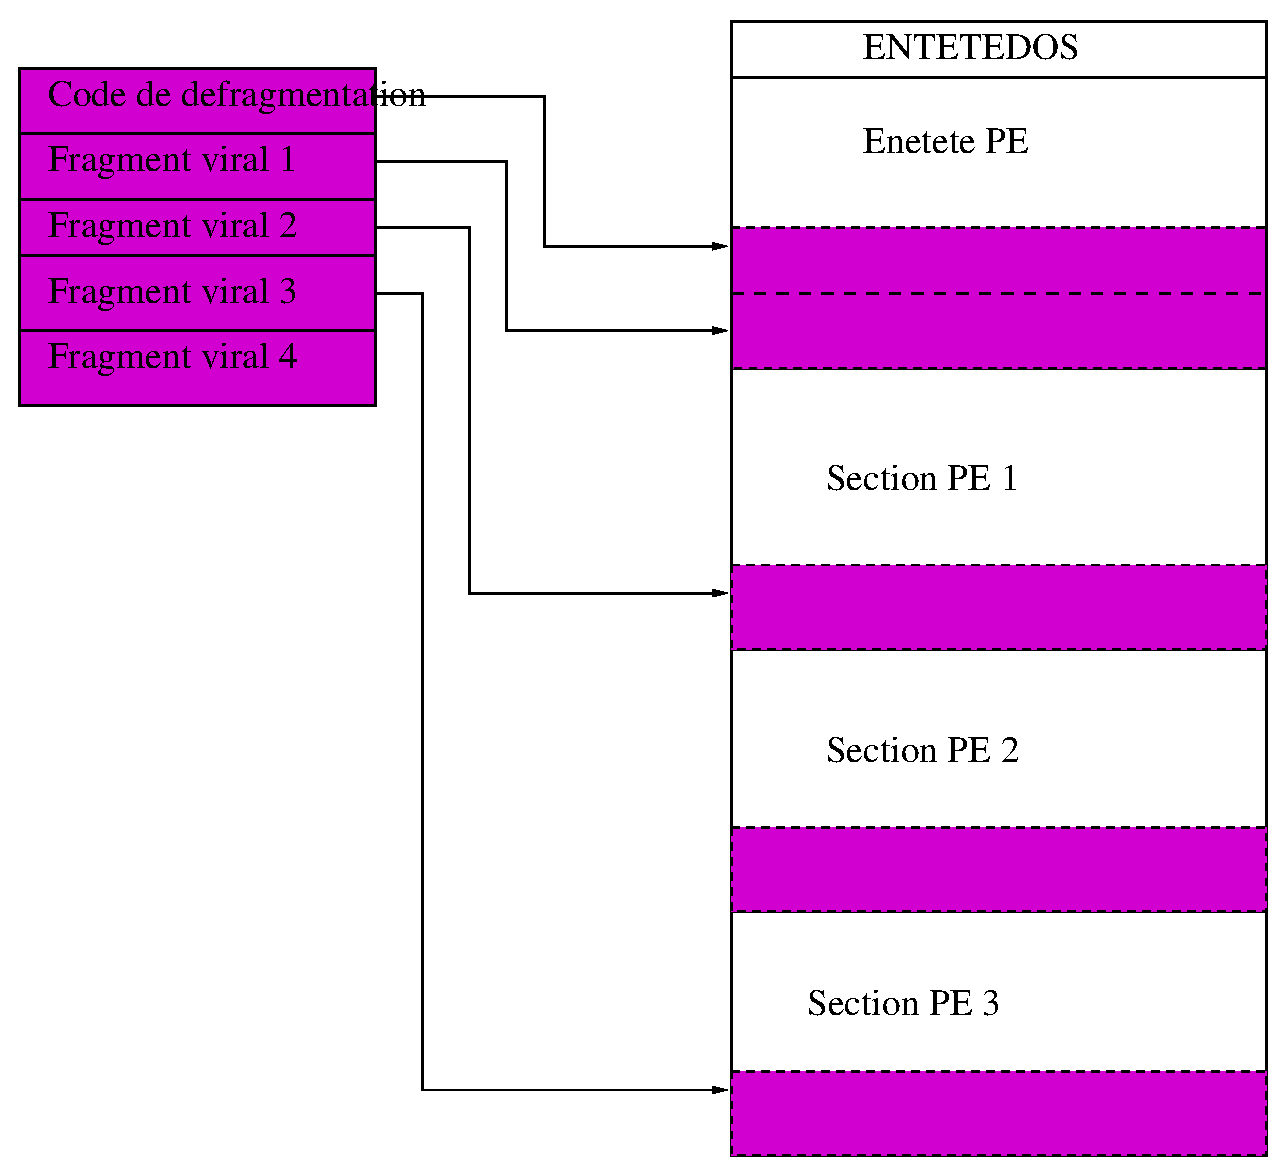
\includegraphics[width=10cm]{entrelacement}
\end{center}

\end{frame}

\subsection{Companion Viruses}

\begin{frame}
\frametitle{Companion Viruses}
\begin{itemize}
\item Least known method.
\item The target code is not altered.
\item The viral code takes the name of the original program and executes the target code using the \texttt{exec} or \texttt{system} command.
\end{itemize}
\begin{center}
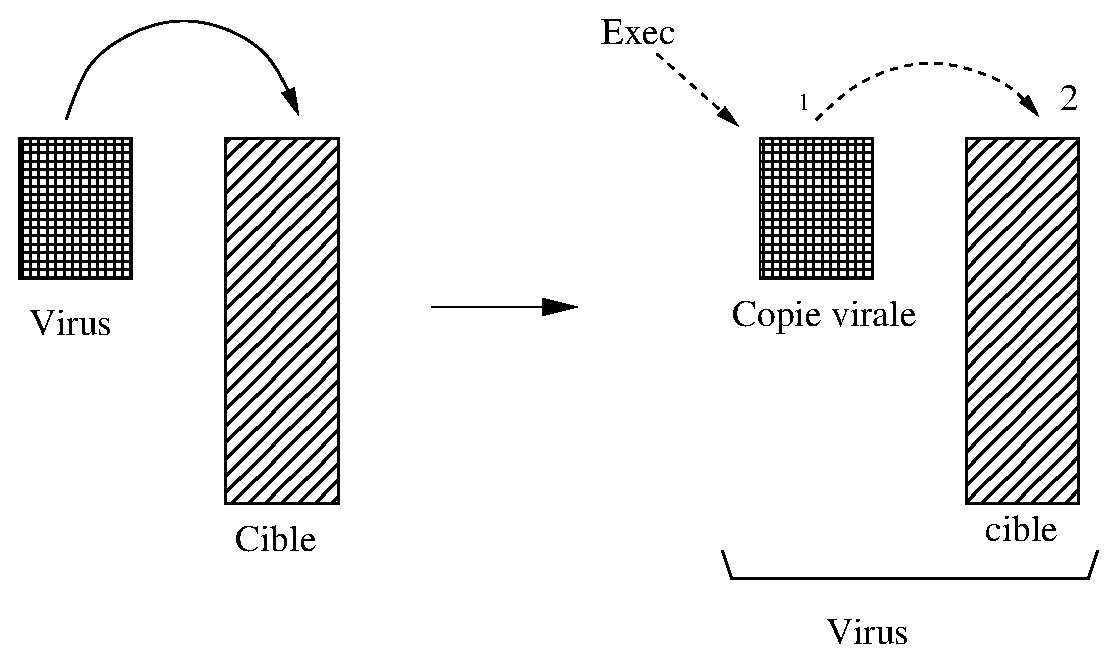
\includegraphics[width=10cm]{accompagnement}
\end{center}

\end{frame}

\begin{frame}
\frametitle{Companion Viruses - Linux Example}

\begin{itemize}
\item On Linux, the virus modifies the PATH by prepending the current directory ``.''.
\item In the current directory, a copy of the virus is made under the name \texttt{ls}.
\item The virus code is modified so that it launches the system \texttt{ls} command at the end of its execution.
\end{itemize}

A similar approach can be used on Windows.
\end{frame}

\subsection{Source Code Viruses}

\begin{frame}
\frametitle{Source Code Viruses}
\begin{itemize}
\item The target here is the source code of a C program.
\item The infected program must be recompiled to produce a valid executable.
\item A quick analysis of the infected code could reveal the presence of the virus, so the code must be duplicated in a more sophisticated manner.
\item The advantage of source code infection is that the resulting binary is completely homogeneous.
\end{itemize}
\end{frame}



\begin{frame}
\frametitle{Source Code Viruses}
\begin{center}
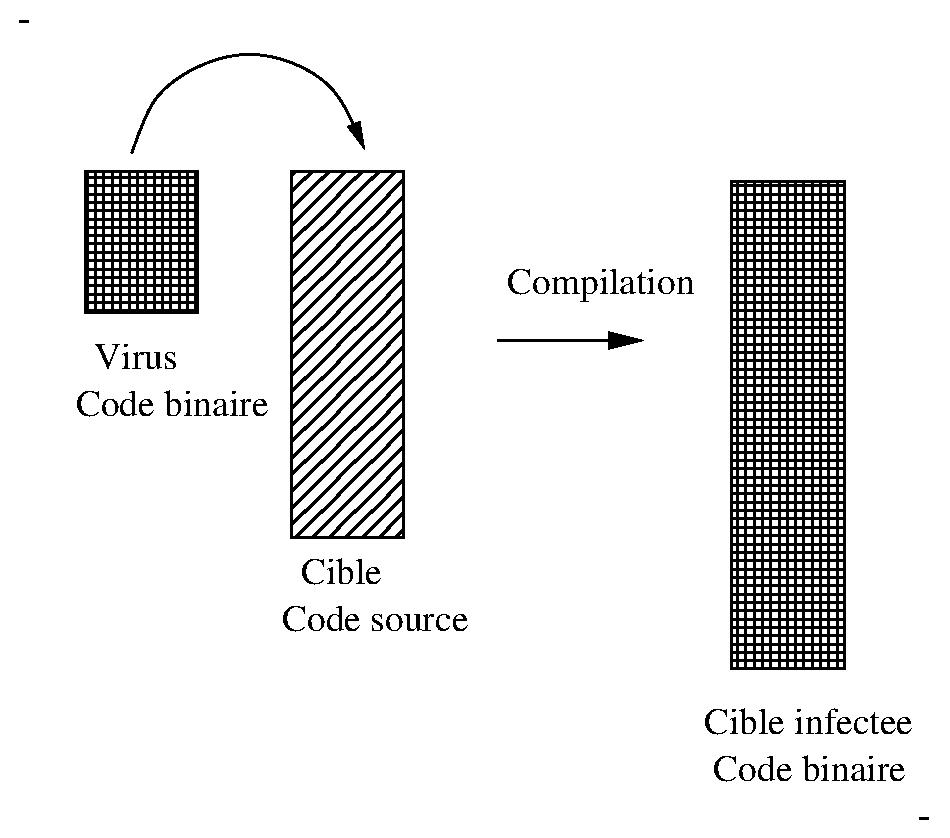
\includegraphics[width=8cm]{viruscodesource}
\end{center}
\end{frame}


\subsection{Anti-Antivirus Techniques}


%\begin{frame}
%\frametitle{Les techniques anti-antivirales}
%\begin{deft}[Sécurité]
%Ensemble  des mesures et techniques destinées à contrer les actions malveillantes contre un système, actions dont la nature propre est s'adapter aux protections qui lui sont opposées.
%\end{deft}
%\end{frame}

\begin{frame}
\frametitle{Anti-Antivirus Techniques}
\begin{itemize}
\item %Dans le cadre de la lutte antivirale, il est alors parfaitement logique que les virus, vers ou autres infections informatiques,
Malware evolves to counter and defeat protections implemented by antivirus software or firewalls.
\medskip

\item  \enlight{Stealth.} Used to deceive the user, the system, and protection software by making them believe there is no malicious code present. % Par exemple en dissimulant le code comme dans l'infection par entrelacement.
\medskip

\item \enlight{Polymorphism.} Since antivirus software largely works by searching for \alert{viral signatures}, the goal of polymorphism is to vary the viral code from copy to copy. %tout élément fixe pouvant être exploité par l'antivirus pour identifier le virus.
\end{itemize}
\end{frame}

\begin{frame}
\frametitle{Anti-Antivirus Techniques: Polymorphism}

The two main techniques are as follows:


\begin{itemize}
\item Code rewriting using equivalent code. For example in C language:
\begin{flushleft}
\begin{tt}
if( flag ) infection();
else payload();
\end{tt}
\end{flushleft}
can be rewritten as follows:
\begin{flushleft}
\begin{tt}
(flag) ? infection() : payload();
\end{tt}
\end{flushleft}
\medskip

\item Using basic encryption techniques on all or part of the virus or worm. %En général, il s'agit plus d'un procédé de masquage (XOR bit à bit) avec une valeur constante.

%Le code viral commence par une procédure en clair dont le but est de déchiffrer le reste du code. Il est alors nécessaire de changer à chaque infection de procédure de chiffrement.

\end{itemize}
\end{frame}



\section{Virus and Worm Classification}


\subsection{Virus Classification}
\begin{frame}
\frametitle{Virus Classification}
Viruses and worms can be classified according to different criteria:
\begin{itemize}
\item by target format: {\color{blue} executable} viruses or {\color{blue} document} viruses.
\item by target component: {\color{blue} boot sector viruses, device driver} viruses,\ldots.
\item by programming language: assembly viruses, source code viruses, script viruses.
\item by behavior: armored viruses, slow or fast viruses, retroviruses, resident viruses, polymorphic or stealth viruses,\ldots
\end{itemize}
\end{frame}



%\begin{frame}
%\frametitle{Virus d'exécutable}
%\begin{itemize}
%\item L'infection concerne une cible binaire à partir d'un fichier binaire infecté. 
%\item Il s'agit en général de mécanisme de bas niveau qui obligent, en règle générale, à utiliser l'assembleur.
%\end{itemize}

%Les cibles principales sont les suivantes
%\begin{itemize}
%\item Les fichier \texttt{*.COM} qui sont de taille $<  64KO$, donc un seul segment mémoire. La contrainte forte lors de l'infection est de garder un binaire $< 64KO$.
%\item Exécutable \texttt{*.EXE}, on a vu les stratégies possibles dans la section précédentes (entrelacement, accompagnement, etc.).
%\item Fichier exécutables au format ELF (Unix). 
%\end{itemize}
%
%C'est le format de ces fichiers qui va dicter le mécanisme d'action du virus.
%\end{frame}


\begin{frame}
\frametitle{Document Viruses or Macro Viruses}
We will adopt the following definition:

\begin{deft}[Document Viruses]
A document virus is:
\begin{itemize}
\item Viral code contained in a {\color{blue} data file, non-executable.}
\pause
\item It is activated by {\color{blue} an interpreter} natively contained in the application associated with the file format (determined by its extension).
\pause
\item The malicious code activation is performed:
\begin{itemize}
\item either by a feature provided in the application,
\item or by exploiting an internal vulnerability of the application.
\end{itemize}
\end{itemize}
\end{deft}

\end{frame}


%\begin{frame}
%\frametitle{Virus de document ou macro virus.}
%On évalue le risque lié à l'infection d'un document lié au condition d'exécution du code du document. 
%\begin{enumerate}
%\item Le format de fichier contient toujours du code, qui est directement exécuté à l'ouverture du fichier.
%\item Le format contient parfois du code, qui  peut s'exécuter directement.
%\item Le format contient parfois du code qui ne s'exécuter qu'après confirmation de l'utilisateur.
%·\item  Le format contient parfois du code qui ne peut s'exécuter qu'après une action volontaire de l'utilisateur.
%\item Le format ne peut jamais contenir le code.
%\end{enumerate}
%\end{frame}



\begin{frame}
\frametitle{Document Viruses: Risks Associated with Known Formats}
\begin{center}
\begin{small}
\begin{tabular}{|c|c|c|c|}
\hline
Format & File Extensions & Risk & Type \\
\hline
\hline
WSH Script & VBS,JS,VBE,JSE,WSF,WSH & 1 & text \\
\hline
Word & DOC,DOT,WBK,DOCHTML & 2,3, & binary \\
\hline
Excel & XLS,XL?,SLK,XLSHTML & 2,3 & binary \\
\hline
Powerpoint & PPT, POT,PPS, & 2,3 & binary \\
 & PPA,PWZ,PPTHTML, POTHTML & & \\
\hline
Access & MDB,MD?,MA?,MDBHTML & 1 &binary \\
\hline
RTF & TRTF & 4 & text \\
\hline
Shell Scrap & SHS & 1 & binary \\
\hline
HTML & HTML,HTM,\ldots & 2 & text\\
\hline
XHTML & XHTML,XHT,\ldots & 2 & text\\
\hline
Adobe Acrobat & PDF & 2 & text \\
\hline
PostScript & PS & 1,2 & text \\
\hline
tex,latex & TEX & ? & text \\
\hline
\end{tabular}
\end{small}
\end{center}
\end{frame}



%\begin{frame}
%\frametitle{Virus de document - Statistique}

%\begin{itemize}
%\item Les formats les plus touché par les infections sont ceux de la suite Office de Microsoft.
%\item Cela s'explique en partie par la popularité de ces logiciels et formats de fichiers.
%\item Statistique (ci-dessous) des attaques sur les différentes version de la suite office.
%\end{itemize}


%\begin{center}
%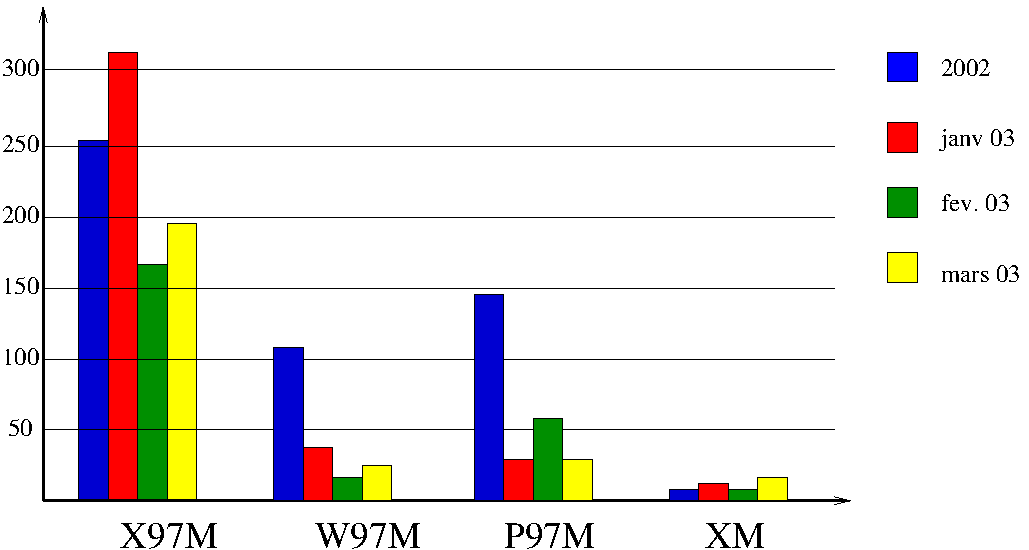
\includegraphics[width=7cm]{stat-macro-virus}
%\end{center}

%\end{frame}



\begin{frame}
\frametitle{BIOS Viruses - Boot Sector Viruses}
\noindent  {\color{blue} BIOS Viruses:}
\begin{itemize}
\item When the computer is powered on, the code contained in the BIOS is activated.
\item Its role is to test the hardware environment and then pass control to the boot sector.
\item A BIOS virus modifies the BIOS code.
\end{itemize}
\noindent {\color{blue} Boot Sector Viruses:}
\begin{itemize}
\item The viral code is placed in the boot sector of the hard drive.
  \item It executes before any other program, allowing it to disable antivirus protection before it runs.
  \end{itemize}
\end{frame}

%\begin{frame}
%\frametitle{Virus de Bios}
%Un virus BIOS présente plusieurs avantages fondamentaux
%\begin{itemize}
%\item il n'est détecté par aucun antivirus. Ces derniers surveillent au niveau du BIOS le secteur de démarrage maître et au niveau du système d'exploitation le disque dur et l'activité système. Aucun contrôle du BIOS lui même n'est effectué.

%\item du fait de son antériorité de lancement, tout programme situé au niveau du Bios ou lancé par lui peut agir sur les données présentes sur la disque.
%\item  Tout programme lancé par le Bios accède à n'importe quelle donnée sur le disque sans limitation. Les possibilités en terme d'infection et de charges finales sont sans limite.

%\end{itemize}
%\end{frame}

%\begin{frame}
%\frametitle{Virus de démarrage}
%Le virus se copie dans le secteur de démarrage : 
%\begin{itemize}
%\item Le secteur de démarrage maître (Master Boot Record ou MBR) prend le relais du Bios. 
%\item Son rôle est de lancer l'un des systèmes d'exploitation présents sur le disque. 
%\item Ce secteur est un exécutable de 512 octets.
%\end{itemize}
%L'intérêt du virus de démarrage est de s'exécuter avant tout autre programme
%Comme dans le cas du virus de BIOS, l'intérêt du virus de démarrage est de s'exécuter avant tout autre programme (hors BIOS) dont un éventuel antivirus. 

%\end{frame}

%\begin{frame}
%\frametitle{Virus de démarrage}
%Deux techniques d'infection du secteur de démarrage existent
%\begin{enumerate}%
%\item Le virus est en réalité un secteur de boot viral, 
%\begin{itemize}
%\item Il écrase et remplace le secteur original sain. 
%\item Il possède toutes les fonctionnalités d'un programme de démarrage en y incluant les capacités virales. 

%\item Cela limite les fonctionnalité du virus (faible taille du code).
%\end{itemize}

%\item Virus plus complexes, possédant des fonctionnalités plus évoluées (furtivité, charge finale) la taille du virus dépasse largement la taille d'un secteur de démarrage

%\begin{itemize}
%\item Le secteur de démarrage viral SDV qui va venir remplacer le secteur de démarrage original sain.
%\item Plusieurs secteurs additionnels viraux. Ces secteurs sont généralement dissimulés ou chiffré. C'est le secteur SDV qui rassemblera ces secteur disséminé lors de l'exécution.
%\item Une copie du secteur de démarrage sain. Le virus une fois l'installation en mémoire effectuée pour pouvoir infecter d'autres secteurs de démarrage redonne le contrôle au secteur original sain qui  lancera le système d'exploitation. 
%\end{itemize}

%\end{enumerate}
%\end{frame}


\begin{frame}
\frametitle{Memory-Resident Viruses}
This is a virus that is {\color{blue} constantly running.}
\begin{itemize}
\item A resident virus is a virus that, once executed, remains active: only shutting down the machine or a \texttt{kill} command can stop it.
\item It uses various techniques to be re-executed after a machine shutdown (launch at startup, etc.).
\item It can interfere with the system (bypass certain system interrupts, for example).
\end{itemize}
\end{frame}


%\end{document}

%\begin{frame}
%\frametitle{Virus lents - Virus rapides}


%Ces virus en fait sont le plus souvent de simples virus d'exécutables, dont l'infection utilise une des techniques de la section précédente.

%\begin{itemize}
%\item les virus lents, en mode résident, n'infectent que les fichiers exécutables qui sont modifiés ou créés.  Le but est de leurrer les antivirus, notamment ceux fonctionnant par contrôle d'intégrité en faisant passer la modification du code et l'action infectieuse proprement dite comme légitimes.
%\item Les virus rapides au contraire eux aussi résidents infectent cette fois les fichiers qui sont exécutés ou ouverts. Cet événement est fréquent ( d'où le nom de virus rapides), tout particulièrement lors de l'exécution d'un antivirus (ouverture de fichier, recherche de signature et émulation de code). Le virus cette fois emboîte le pas à l'antivirus, et ce dernier ne voit que sa propre action. 
%\end{itemize}
%\end{frame}




\begin{frame}
\frametitle{Virus Hoax}

%C'est un phénomène relativement récents et très particulier: c'est une sorte de duplication de code social.
This is a kind of viral code that executes in the brain.
\bigskip

\begin{definition}[Virus Hoax]\begin{itshape}
A \enlight{virus hoax} is misinformation that uses social engineering techniques to induce users to produce effects equivalent to those of a virus or worm: propagation and offensive action.
\end{itshape}
\end{definition}

\bigskip
{\color{blue} Example:} circulation of an email warning of an infection, solved by deleting a system file.

\end{frame}




\subsection{Worm Classification}


\begin{frame}
  \frametitle{Classification}
 \noindent {\color{blue} Simple Worms:}
\begin{itemize}
\item These are the ones that can legitimately be called worms.
\item They generally exploit software and network vulnerabilities allowing program execution on a remote machine.
%\item Ils exploitent aussi des faiblesses dans les protocoles réseaux (mots de passe faible, authentification sur l'IP,\ldots).
\end{itemize}
\noindent {\color{blue} Macro Worms (virus-worm hybrids):}
\begin{itemize}
\item Dissemination occurs through attachments containing infected office documents sent to users in the address book.
\end{itemize}
\noindent {\color{blue} Email Worms:}
\begin{itemize}
\item Propagation through attachments containing malicious code.
\item The code is activated either by the user or by the email application.
  \item The most famous example is the ILOVEYOU worm.
  \end{itemize}
\end{frame}

%\end{document}

%\section{La lutte antivirale}


\section{Conclusion}

\begin{frame}
  \frametitle{Key Takeaways}
  This chapter provides general information about malware:
  \begin{itemize}
  \item Understand the different types of malware.
  \item Distinguish between viruses and worms.
  \item Understand virus replication methods.
    \item Understand virus propagation methods.
    \end{itemize}
\end{frame}
\end{document}
